\section{Introduction} \label{sec:intro}

\indent Give a brief introduction to this subject. Talk about the background, as well as what our main goal
of doing this project is. This is an example of a citation, see Ref.\cite{cyero_phdthesis}
This is an example of a Figure:\\
\begin{figure}[h!]
  \centering
  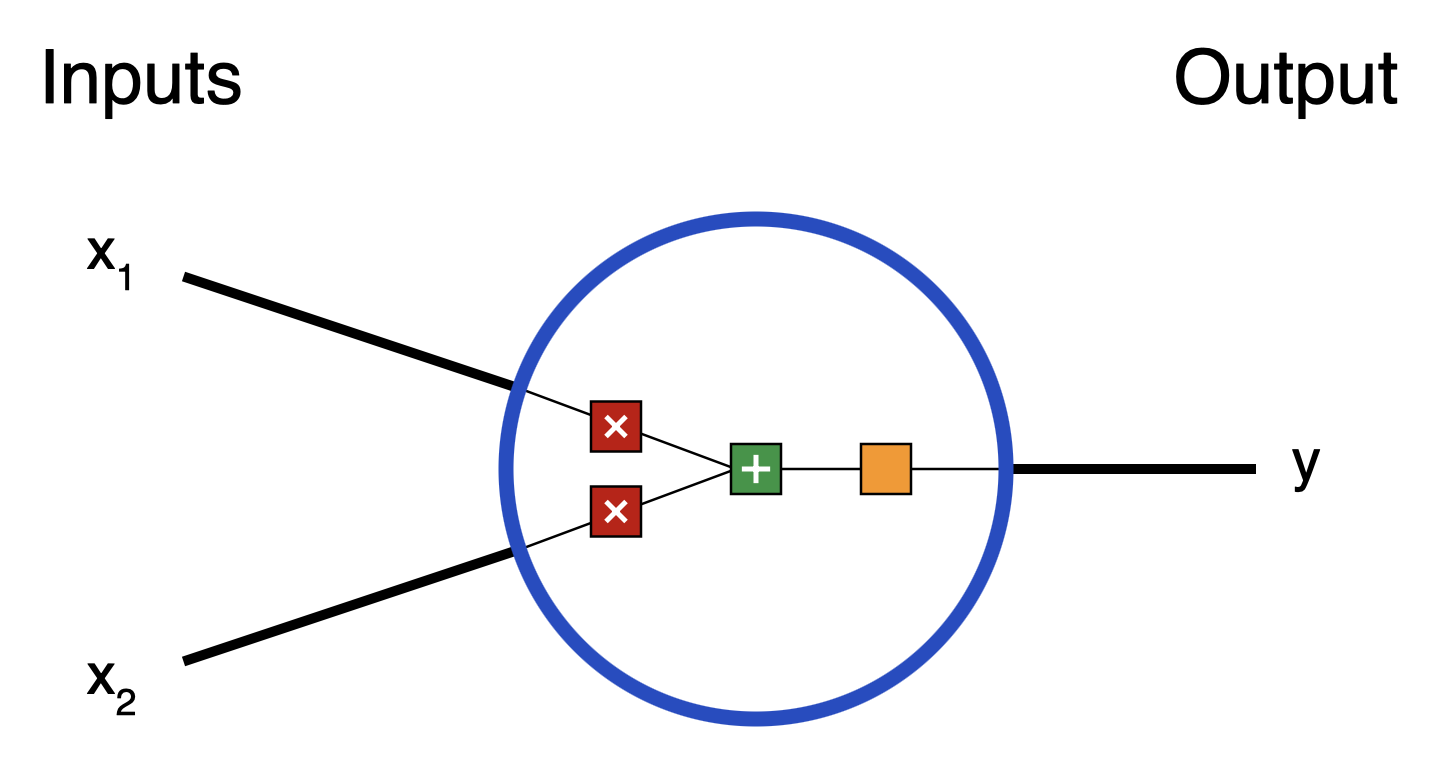
\includegraphics[scale=0.3]{sections/images/Neuron.png}
  \caption{This is a description/caption of the image. Image Source: See \cite{VZhou_blog_NN_intro}}
  \label{fig:Neuron}
\end{figure}
This is an example of how to reference the figure, see Fig.\ref{fig:Neuron}.
An example of how to cite another section, see Section \ref{sec:conclusion}

An example of an Equation,
\begin{equation}
  f(x)  = \frac{1}{1 + e^{x}}
  \label{eq:1}
\end{equation}

See Eq. \ref{eq:1}
